\providecommand{\StudySection}{\section}
\providecommand{\StudySubsection}{\subsection}

\StudySection{Choosing how many Kira workers to use}
\label{sec:thread-policy}
The ordering study gives no further saving, so we retain the seed-expansion method and its earlier ordering. We next test the number of Kira workers, which determines how much of the symbolic calculation can run in parallel~\cite{KiraOriginal}. Development measurements show that extra workers add overhead on small batches, while some larger box batches finish sooner. This suggests choosing the worker count from the requested targets before equation generation.

The candidate counts are one, two, and four workers in the same integrated executable. The native control uses Kira's own seed and reduction decisions together with the common earlier implementation changes. For the learned comparison, the nine target features used above predict each worker count's complete time relative to one worker. We fit ten predictor types per graph on 36 training batches, select settings on 18 validation batches, and reserve 36 more batches for testing. Validation minimizes the sum of batch median times. A predictor must save at least two percent against the faster control and give lower summed time in at least two of three validation repetitions; otherwise the control remains active. Appendix~\ref{app:thread-policy} gives the labels, checks, and comparison rules.

Validation enables a depth-two tree for the planar box and a depth-one tree for the nonplanar box. The other five graph types retain the preceding one-worker strategy. Both trees split only on the number of targets in the batch and choose at most two workers. Since the tested target patterns repeat across the parameter splits, these results establish a useful decision within those patterns; they do not establish target count as a sufficient description of arbitrary integral structures. Training and validation contain 1,098.1 seconds of reductions, and fitting all seventy candidates takes 0.82 seconds. These offline costs exclude reference construction and development.

All 900 timed reductions and 50 additional applications pass exact checks. The additional applications receive targets and a prescribed basis without reference coefficients. Seven run consecutively through a caller that keeps the models loaded, in a separate two-core allocation; each native attempt still starts a fresh Kira process. The timing experiment reserves four cores for every method so that the always-four-worker control can use its full setting. Thus every timed method has the same available resources, even when it uses fewer workers.

For the 36 reserved batches, the sum of median complete times falls from 82.21 seconds with the preceding one-worker method to 78.73 seconds with worker selection, a reduction of 4.2\%. In the same experiment, native one-worker choices take 110.67 seconds, always using four workers takes 156.95 seconds, and a fixed count for each graph takes 82.45 seconds. Selection therefore gives 4.5\% less time than the fixed-per-graph control. Table~\ref{tab:thread-policy} shows where these differences arise; changes for the five graphs that retain one worker include execution variation and the additional decision cost.

\begin{table}[!htbp]
\centering\small
\caption{Time with and without worker selection. Entries sum the batch median times within each graph, in seconds. ``Previous'' uses the seed-expansion method with one worker; ``Selected'' uses the validation-selected count. The final column divides selected time by previous time.}
\label{tab:thread-policy}
\begin{tabular}{@{}llrrr@{}}\toprule
Graph & Choice & Previous (s) & Selected (s) & Selected/previous\\\midrule
Sunrise & 1 worker & 5.271 & 5.215 & 0.989\\
Planar box & Tree depth 2 & 15.643 & 14.997 & 0.959\\
Vacuum & 1 worker & 4.813 & 4.620 & 0.960\\
Ladder & 1 worker & 23.197 & 23.602 & 1.017\\
Nonplanar box & Tree depth 1 & 26.768 & 23.819 & 0.890\\
Pentagon & 1 worker & 3.558 & 3.523 & 0.990\\
Virtuality box & 1 worker & 2.963 & 2.955 & 0.997\\
\bottomrule\end{tabular}
\end{table}

Giving each graph equal weight yields a smaller selected-to-preceding ratio of $0.9817$, with descriptive interval $[0.9682,0.9946]$, or 1.8\% less time. The selected-to-native ratio is $0.8456$ with interval $[0.7346,0.9502]$, or 15.4\% less time. These averages give equal importance to each graph, whereas the sum of medians measures the time for this particular collection of requests. Figure~\ref{fig:thread-policy} also shows why simply increasing every calculation to four workers is ineffective on these small cases.

\begin{figure}[!htbp]
\centering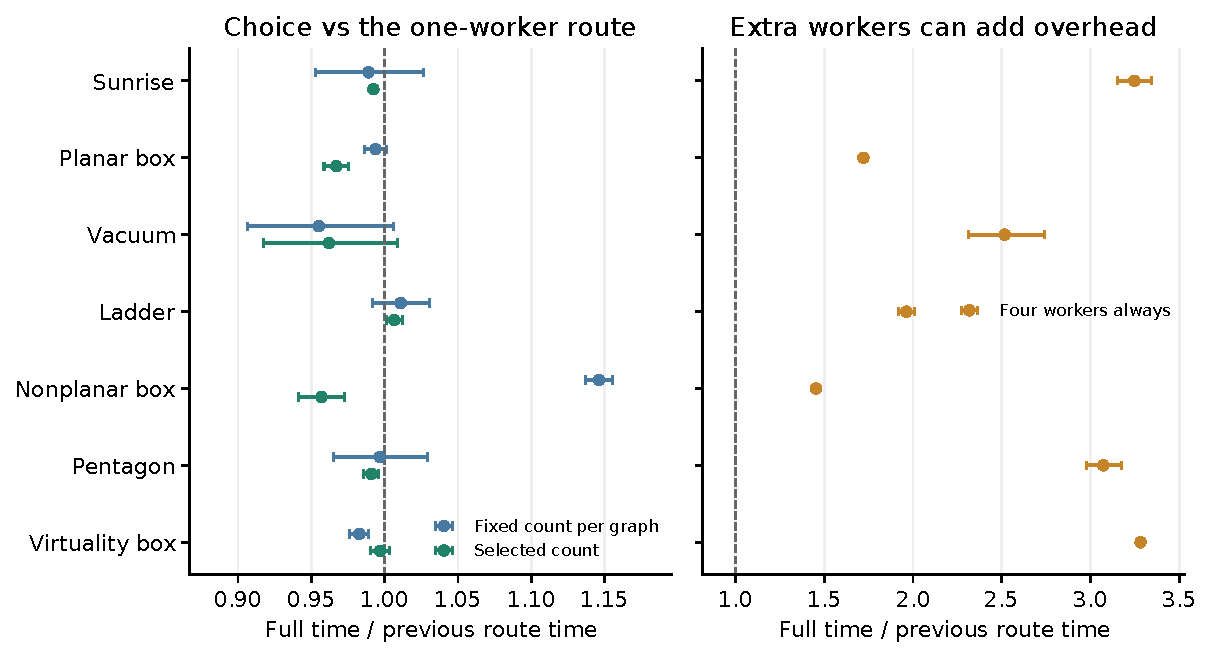
\includegraphics[width=\linewidth]{paper_figures/thread_policy.pdf}
\caption{The effect of selecting the worker count. Left: selected and fixed worker counts compared with the preceding
one-worker method. Right: always using four workers adds overhead on
many small cases. Each panel has its own horizontal scale.
Each point is the geometric mean of batch time ratios for one graph. Bars show the
range across two parameter profiles and are not significance intervals.}
\label{fig:thread-policy}
\end{figure}

\FloatBarrier

Variation between repetitions matters for the size of the gain. Across all five repetitions, the selected method takes 404.84 seconds and the preceding method 414.08 seconds, giving 2.2\% less elapsed time. Selection has lower summed time in four of the five repetitions, with selected-to-preceding ratios ranging from $0.9346$ to $1.0555$. This range describes the observed repetitions and is not a confidence interval. The ladder's sum of median times increases by 1.7\%.

The saving in elapsed time also uses more CPU time. The extra prediction takes a median of 276.6 microseconds and is included in the complete-time measurements. Across 180 reductions per method, the preceding strategy uses 385.9 CPU-seconds, the always-four-worker strategy 1024.1, and the selected strategy 458.9. Selection therefore increases CPU use by 18.9\%. These values measure CPU time consumed by the calculation, rather than the number of cores allocated to it.

The selected method has no failed attempts and requires no fallback. The always-four-worker method has ten unsuccessful native attempts, whose subsequent retries succeed; their costs remain in the reported time. Some native attempts report allocation failures under the imposed process limits. All comparisons include prediction, preparation, exact algebra, basis conversion, checks, retries, and cleanup, with the caller and models loaded before timing and a fresh Kira process for each attempt.

Worker selection is retained for this measured workload because it lowers elapsed time while preserving the exact results. Its demonstrated scope is seven known graph structures at one through three loops, known target patterns, and new rational kinematics with symbolic dimension. The preceding one-worker method remains available when the resource conditions or inputs differ. The result identifies a measured improvement among the tested choices, with the CPU cost stated alongside it.
